% This is samplepaper.tex, a sample chapter demonstrating the
% LLNCS macro package for Springer Computer Science proceedings;
% Version 2.20 of 2017/10/04
%
\documentclass[runningheads]{llncs}
%
\usepackage{graphicx}
\usepackage{hyperref}
\usepackage{xcolor}
\usepackage{tabularx}
\usepackage{subcaption}
\usepackage{longtable}
\usepackage{threeparttablex}
\usepackage{booktabs}

\newcolumntype{C}{>{\centering\arraybackslash}X}
% Used for displaying a sample figure. If possible, figure files should
% be included in EPS format.
%
% If you use the hyperref package, please uncomment the following line
% to display URLs in blue roman font according to Springer's eBook style:
% \renewcommand\UrlFont{\color{blue}\rmfamily}

\begin{document}
%
\title{GSSSP\,: Generator of Synthetic Scans of Spectroscopic Plates for Object Detection}
%
\titlerunning{GSSSP}
% If the paper title is too long for the running head, you can set
% an abbreviated paper title here
%
\author{
    Santiago Andres Ponte Ahón\inst{1}\orcidID{0009-0002-8540-6546} \and
    Juan Martín Seery\inst{1}\orcidID{0009-0005-3009-8330} \and
    Facundo Quiroga\inst{1,2}\orcidID{0000-0003-4495-4327} \and
    Franco Ronchetti\inst{1,2}\orcidID{0000-0003-3173-1327} \and
    Yael Aidelman\inst{3,4}\orcidID{0000-0001-5279-0241} \and
    Waldo Hasperué\inst{1}\orcidID{0000-0002-9950-1563} \and
    Roberto Gamen\inst{3,4}\orcidID{0000-0002-5227-9627} \and
    Lydia Cidale\inst{3,4}\orcidID{0000-0003-2160-7146}
}
%
\authorrunning{S. Ponte Ahón et al.}
% First names are abbreviated in the running head.
% If there are more than two authors, 'et al.' is used.
%
\institute{
    Instituto de Investigación en Informática LIDI, Universidad Nacional de La Plata, La Plata, Argentina\\
    \email{\{sponte,jmseery,fquiroga,fronchetti,whasperue\}@lidi.info.unlp.edu.ar}\\ 
    \url{https://weblidi.info.unlp.edu.ar/} \and
    Comisión de Investigaciones Científicas de la Provincia de Buenos Aires (CICPBA), Buenos Aires, Argentina \\
    \url{https://www.cic.gba.gob.ar/} \and
    Facultad de Ciencias Astronómicas y Geofísicas, Universidad Nacional de La Plata, La Plata, Argentina \\
    \email{\{aidelman,rgamen,lydia\}@fcaglp.unlp.edu.ar}\\
    \url{https://www.fcaglp.unlp.edu.ar/} \and
    Instituto de Astrofísica de La Plata, La Plata, Argentina \\
    \url{https://ialp.fcaglp.unlp.edu.ar/}
}
%
\maketitle              % typeset the header of the contribution
%
\begin{abstract}
    GSSSP (Generator of Synthetic Scans of Spectroscopic Plates) is a tool for generating labeled scans of physical spectroscopic observations.
    The area of spectroscopic analysis is old in the Astronomic Domain. Legacy observational methods recorded stellar spectra on photographic plates. These plates have high historical and scientific value. However, a limited number of them have been digitized, resulting in an insufficient amount of data to train modern computer vision models for observation detection.
    
    In this work, we present a software tool that replicates the appearance of scanned spectroscopic plates by generating synthetic images containing spectra of artificial stellar objects. The generated images are accompanied by label files that enable the training of observation detection models.
    
    We trained a detection model and compared its performance when using only real data, only generated data, and a combination of both. The results show that GSSSP enables the model to learn the general visual patterns of this type of plate, providing a strong generalization basis for subsequent fine-tuning. The resulting model surpasses the current state of the art for this problem.
    
    \keywords{Generated data, Object detection, Spectroscopic plates}
\end{abstract}

\section{Spectroscopic Data}

Spectroscopy constitutes a fundamental tool for physic study of astronomical objects. The analysis of electromagnetic radiation receibed, absorbed, or reflected is posible infer physics propieties of objects. By example, quimic composition, temperature, radial speed. This science enable celest bodis study further of her position or apparent brightness~\cite{gray2021observation}. 

In XX century the capture of spectroscopic data was very popular. The method consist in capture spectroscopic data through photography. With the peculiarity what the image persisted in glass plates instead of paper. Today many of these plates are conserved for their institutions~\cite{kunzmann2009real}. However, the persistence of data in physical plates can present problems under suboptimal storage conditions. Figure~\ref{fig:glass_plate} show a spectroscopic glass plate with two observations in its surface.

\begin{figure}[htb!]
    \centering
    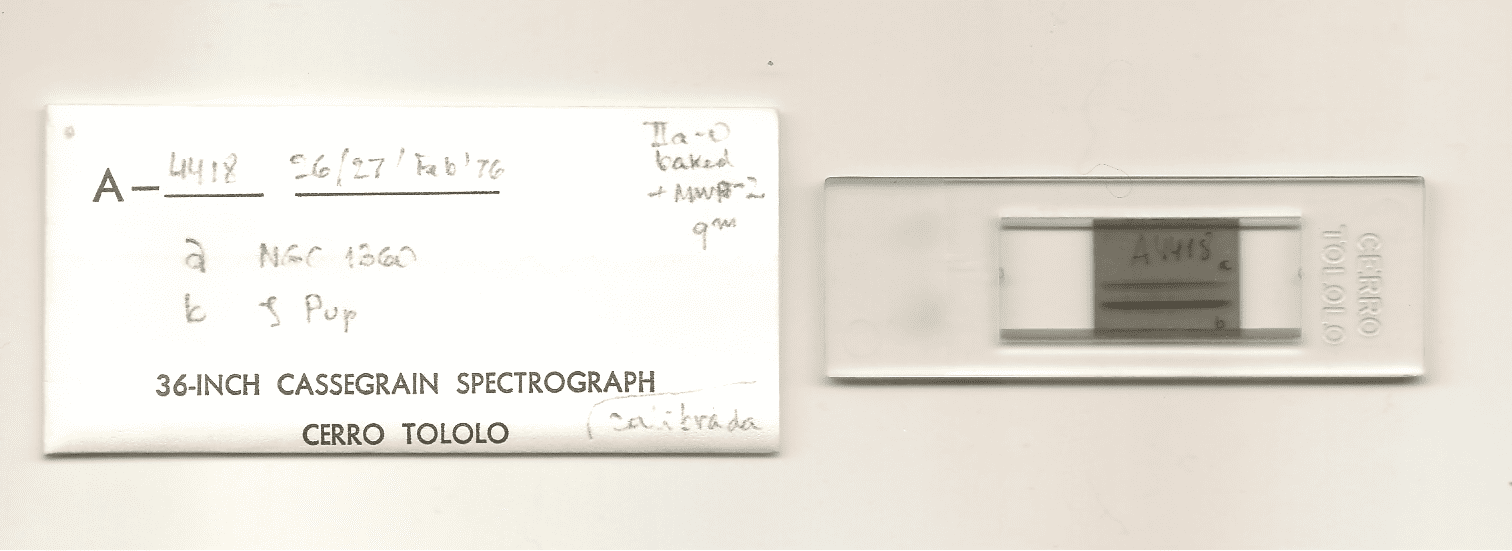
\includegraphics[width=1\textwidth]{images/glass-plate.png}
    \caption{
        Right, spectroscopic plate \texttt{A4418} of astronomical source \texttt{Zeta Puppis} captured at Observatorio Interamericano de Cerro Tololo (Chile) as part of the \texttt{ReTrOH}~\cite{niemela1977placa} project. The plate contains two spectroscopic observations. Left, wrapping, includes additional information about each observation.
    }\label{fig:glass_plate}
\end{figure}

Accidents have occurred in involving this type of heritage. In 2016, due a burst pipe, Hardvard College Observatory suffered a flood that affected more than 61.000 plates in its colection~\cite{placas_DASCH}. Too, Facultad de Ciencias Astronomicas y Geofisicas de la Universidad Nacional de La Plata found an equally damaging situation, discovering mold on the furniture where the plaques were stored~\cite{peralta2025puesta}. 
The risk of mold stains, scratches, cobwebs, or similar problems is significant and, if not properly addressed, can lead to consequences that permanently degrade the information available on each plate.

In addition to physic deterioration can be introduced defects exist defects related to the capture process such as curvatures in the trace of the spectra, artifacts, or the loss of certain elements. Figure~\ref{fig:defectos_placas} show refences of plates with some defect.

\begin{figure}[htb!]
    \centering
    \begin{subfigure}[b]{0.30\textwidth}
        \centering
        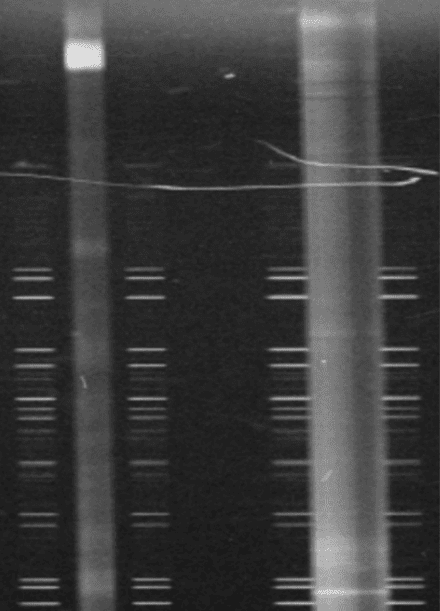
\includegraphics[height=5cm]{images/defecto_rayon.png}
        \caption{}
    \end{subfigure}
    \hfill
    \begin{subfigure}[b]{0.12\textwidth}
        \centering
        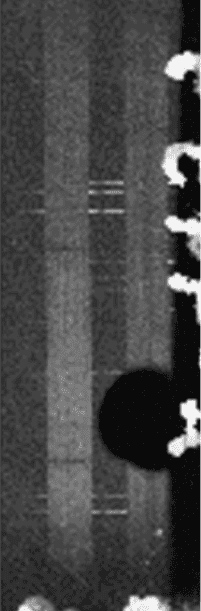
\includegraphics[height=5cm]{images/defecto_humedad.png}
        \caption{}
    \end{subfigure}
    \hfill
    \begin{subfigure}[b]{0.12\textwidth}
        \centering
        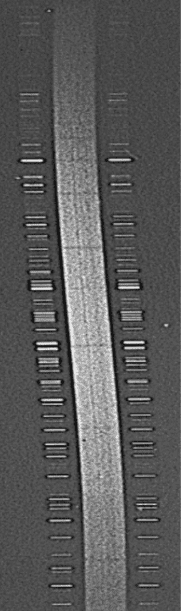
\includegraphics[height=5cm]{images/defecto_curvo.png}
        \caption{}
    \end{subfigure}
    \hfill
    \begin{subfigure}[b]{0.10\textwidth}
        \centering
        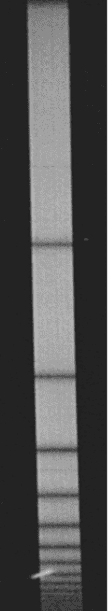
\includegraphics[height=5cm]{images/defecto_falta_lampara.png}
        \caption{}
    \end{subfigure}
    \hfill
    \begin{subfigure}[b]{0.10\textwidth}
        \centering
        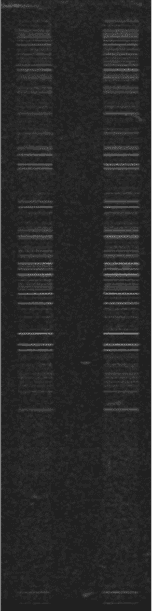
\includegraphics[height=5cm]{images/defecto_falta_espectro.png}
        \caption{}
    \end{subfigure}
    \caption{
        Samples of possible defects on the plates. Defects associated with prolonged storage: (a) Scratches. (b) Dirt and/or moisture stains. Defects associated with the capture process: (c) Curved engraving. (d) Missing comparison lamps. (e) Comparison lamps without their respective spectrum.
        }\label{fig:defectos_placas}
\end{figure}

For preserve this heritage and institutions as IAU (International Astronomical Union) prensented resolutions\footnote
{\href{http://www.iau.org/static/publications/ib88.pdf}{UAI Resolution B3 (Agosto 2000): Safeguarding the Information in Photographic Observations}}. when remark the importance of keep spectroscopic plates for next generations of astronomers. IAU recommends digitalization as conservation method. This methods enable copying facilities and redundancies that can preserve the most relevant information in the long term.

For advance in this many institutions begin projects of digitalization of their collections. Table~\ref{tab:colecciones} list many collections with big count of spectroscopic collections. Theirs digitalization percents and his calibration percents.


\newcolumntype{G}[1]{>{\centering\arraybackslash}p{#1}}
\begin{ThreePartTable}

    \begin{TableNotes}
        \item[a] Solo se calibraron las placas fotográficas.
        \item[b] \textit{Pulkovo Photographic Plate Database (Noviembre 2025)}. Disponible en \url{https://www.puldb.ru/db/plates/}.
        \item[c] \textit{Ukrainian Virtual Observatory, AO KNU DA (Noviembre 2025)}. Disponible en \url{http://ukr-vo.org/digarchives/index.php?b4&1}.
        \item[d] \textit{Ukrainian Virtual Observatory, AO LNU DA (Noviembre 2025)}. Disponible en \url{http://ukr-vo.org/digarchives/index.php?b3&1}.
    \end{TableNotes}

    \begin{longtable}{@{} p{3.7cm} r r r r G{2.5cm} @{}}
        \toprule
        Colección & \#plt.fot. & \#plt.spe. & Digitalizado & Calibrado & Rango\\
        \midrule
        \endhead%

        \midrule[\heavyrulewidth]
        \multicolumn{6}{r}{\textit{continúa en la página siguiente}}\\
        \endfoot%

        \midrule[\heavyrulewidth]
        \insertTableNotes%
        \endlastfoot%

        \texttt{HCO} & $\sim$\,430.000 & $0$ & $100\%$ & $89\%$ & 1880--1992 \\ 
        \nopagebreak
        \multicolumn{6}{l}{\cite{placas_DASCH}} \\\addlinespace
        \texttt{APPLAUSE} & 93.774 & 19.240 & 100$\%$ & 83\%$^{(a)}$ & 1893--1999 \\% Referencia a importancia de las placas del emisferio sur (see Tsvetkova et al. 2018, for detail). % Placas de espectro solo digitalizadas % Todas las espectroscopicas vienen de Hamburg y Potsdam archives. % Hay una referencia en summary que habla del protocolo de calibracion que establecieron los de Hamburg.
        \nopagebreak
        \multicolumn{6}{l}{\cite{placas_APPLAUSE}} \\\addlinespace
        \texttt{CPDP} & 30.750 & 0 & $95\%$ & $51\%$ & 1901--1999 \\ % Placas no digitalizadas <-- defectos en las placas
        \nopagebreak
        \multicolumn{6}{l}{\cite{placas_SHAO}} \\\addlinespace
        \texttt{MMO} & $>$8.500 & 0 & $94\%$ & $0\%$ & 1913--1993 \\
        \nopagebreak
        \multicolumn{6}{l}{\cite{placas_MMO, placas_MMO_2}} \\\addlinespace
        \texttt{ReTrHO} & ? & $>$15.000 & $4\%$ & $0\%$ & 1920--1980\\ % Placas no digitalizadas <- defectos en las placas
        \nopagebreak
        \multicolumn{6}{l}{\cite{peralta2025puesta}} \\\addlinespace
        \texttt{WFPDB} & 640.000 & ? & $100\%$ & $?\%$ & 1858--2005\\
        \nopagebreak
        \multicolumn{6}{l}{\cite{placas_WFPDB, placas_WFPDB_2}} \\\addlinespace
        \texttt{OCA Archive} & 11.800 & 0 & $100\%$ & $?\%$ & 1935--1996\\
        \nopagebreak
        \multicolumn{6}{l}{\cite{robert2021naroo}} \\\addlinespace
        \texttt{OHP Archive} & 7.300 & 63.500 & $100\%$ & $?\%$ & 1944--1997\\ % Acceptan propuestas de digitalizacion (NAROO, min 200 placas)
        \nopagebreak
        \multicolumn{6}{l}{\cite{robert2021naroo}} \\\addlinespace
        \texttt{Pulkovo Archive}$^{(b)}$ & 46.483 & 0 & $100\%$ & $?\%$ & 1893--2005\\
        \nopagebreak
        \multicolumn{6}{l}{\cite{robert2021naroo}} \\\addlinespace
        \texttt{Foster Archive} & 0 & $>$4.800 & $100\%$ & $?\%$ & 1928--1991\\ % El articulo habla de estrellas Be % Pagina 3 menciona defectos de las placas por clima. % Usan la tarea identify de IRAF % Pag 7 muestran funciones ¿I/O? relacionadas a la misma estrella, probablemente una red neuronal pueda aprovechar estas funciones para saber de que se trata. % Para Clasificar Be podriamos ver si hay una forma de convertir imagenes a espectros y eso ingresarlo a una red neuronal. Los espectros de la imagen probablemente mantengan patrones similares para estrellas Be. % BeSOS como base de datos con informacion detallada de espectros concretos
        \nopagebreak
        \multicolumn{6}{l}{\cite{archive_foster}} \\\addlinespace
        \texttt{HDAP} & $\sim$25.000 & 0 & $100\%$ & $?\%$ & 1880--1999\\
        \nopagebreak
        \multicolumn{6}{l}{\cite{placas_HDAP, db_GAVO}} \\\addlinespace
        \texttt{DFBS} & 0 & 1.874 & $100\%$ & $100\%$ & 1965--1980\\ % Automatizaron la extraccion y no tengo claro como resolvieron la calibracion en longitud de onda
        \nopagebreak
        \multicolumn{6}{l}{\cite{placa_DFBS}} \\\addlinespace
        \texttt{AO KNU}$^{(c)}$ & 20.000 & 0 & $ 22\%$ & $0\%$ & 1898--1996\\
        \nopagebreak
        \multicolumn{6}{l}{\cite{archives_ukranian_observatories}} \\\addlinespace
        \texttt{AO LNU}$^{(d)}$ & 8.000 & 0 & $ 25\%$ & $0\%$ & 1939--1976 \\
        \nopagebreak
        \multicolumn{6}{l}{\cite{archives_ukranian_observatories}} \\\addlinespace
        \bottomrule    
        \caption{
            Varios proyectos y colecciones relevantes de placas fotográficas y espectroscópicas.
        }\label{tab:colecciones}
    \end{longtable}

\end{ThreePartTable}



% Para que una placa sea de utilidad es necesario procesarla, extraer las características más relevantes de aquello que contiene y permitir que investigadores y/o académicos puedan emplear su información en nuevos proyectos. Notar que las colecciones mencionadas en la tabla~\ref{tab:colecciones} involucran 2 tipos de placas, placas fotográficas y placas espectroscópicas. Proyectos como \texttt{DASCH}~\citep{placas_DASCH} o \texttt{CPDP}~\citep{placas_SHAO} trabajan sobre placas fotográficas, procesar este tipo de placas tiene sus propios desafíos pero ya hay una método bien definido mediante el cual se puede lograr su procesado en un tiempo razonable~\citep{raouph2023prospectplatearchivephotometric}. La situación de colecciones como \texttt{ReTrOH}~\citep{Meilan2020} o el archivo \texttt{Foster}~\citep{archive_foster} es más compleja ya que las placas espectroscópicas tienen otra anatomía. No se trata de impresiones fotográficas del objeto astronómico sino de impresiones del espectro de luz del mismo. La figura~\ref{fig:comparacion} muestra una comparativa entre una placa fotográfica y una placa espectroscópica.



\textcolor{red}{Descripcion de las placas, relevancia, contexto de que hay pocas}.

\subsection{Available Data}

For this study, we use a dataset composed of 361 spectroscopic plates from \textcolor{red}{Cerro Tololo} that were scanned and labeled for observation detection. The dataset is publicly available
\footnote{\href{https://drive.google.com/drive/folders/1RnGoeTOMmU03VMEa6nk-sVmuETUE-EBa?usp=sharing}{Observation Detection in Spectroscopic Plates Dataset}}. 
Due to the limited availability of digitized spectroscopic plates, the dataset size is relatively small.

\section{State of Art}

\textcolor{red}{Mencion a trabajos previos donde se construyeron modelos de deteccion para observaciones}.

\section{GSSSP}

\textcolor{red}{En que consiste GSSSP, sus modulos. Caracteristicas principales, personalizacion de observaciones e imagenes de spectros}.

\section{Experiment}

\textcolor{red}{Detalles del entrenamiento, datos usados en cada uno y metricas de evaluacion}.

\subsection{Results}

\textcolor{red}{Resultados de cada entrenamiento}.

\begin{table}
    \caption{Results with real, generated and mix data train.}\label{tab:results}
    \begin{tabularx}{\linewidth}{|C|C|C|C|C|}
        \hline
        data train & data test & $MaP$ & $MaP[IoU=50]$ & $MaP[IoU=75]$\\
        \hline
        \textit{real-train} &  \textit{real-test} & 0.6597 & 0.9114 & 0.6681\\
        \textit{gen} &  \textit{real-test} & 0.6431  & 0.8942 & 0.7675 \\
        \textit{gen+real-train} & \textit{real-test} & 0.9360 & 1.0000 & 1.0000\\
        \hline
    \end{tabularx}
\end{table}

\section{Conclusion}

\textcolor{red}{Conclusions}.

\section{Sample Section}
\subsection{A Subsection Sample}
Please note that the first paragraph of a section or subsection is
not indented. The first paragraph that follows a table, figure,
equation etc. does not need an indent, either.

Subsequent paragraphs, however, are indented.

\subsubsection{Sample Heading (Third Level)} Only two levels of
headings should be numbered. Lower level headings remain unnumbered;
they are formatted as run-in headings.

\paragraph{Sample Heading (Fourth Level)}
The contribution should contain no more than four levels of
headings. Table~\ref{tab1} gives a summary of all heading levels.

\begin{table}
\caption{Table captions should be placed above the
tables.}\label{tab1}
\begin{tabular}{|l|l|l|}
\hline
Heading level &  Example & Font size and style\\
\hline
Title (centered) &  {\Large\bfseries Lecture Notes} & 14 point, bold\\
1st-level heading &  {\large\bfseries 1 Introduction} & 12 point, bold\\
2nd-level heading & {\bfseries 2.1 Printing Area} & 10 point, bold\\
3rd-level heading & {\bfseries Run-in Heading in Bold.} Text follows & 10 point, bold\\
4th-level heading & {\itshape Lowest Level Heading.} Text follows & 10 point, italic\\
\hline
\end{tabular}
\end{table}


\noindent Displayed equations are centered and set on a separate
line.
\begin{equation}
x + y = z
\end{equation}
Please try to avoid rasterized images for line-art diagrams and
schemas. Whenever possible, use vector graphics instead (see
Fig.~\ref{fig1}).

\begin{figure}
    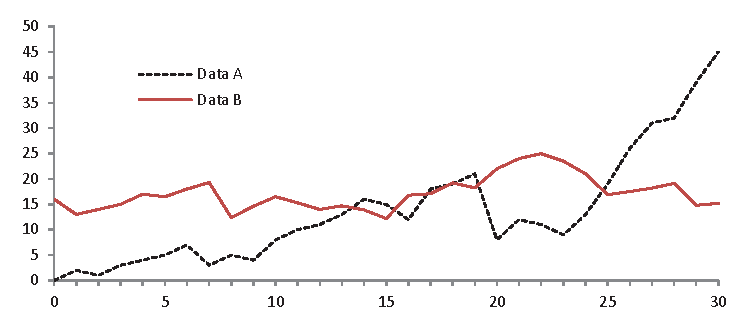
\includegraphics[width=\textwidth]{fig1.eps}
    \caption{A figure caption is always placed below the illustration.
    Please note that short captions are centered, while long ones are
    justified by the macro package automatically.} \label{fig1}
\end{figure}

\begin{theorem}
This is a sample theorem. The run-in heading is set in bold, while
the following text appears in italics. Definitions, lemmas,
propositions, and corollaries are styled the same way.
\end{theorem}
%
% the environments 'definition', 'lemma', 'proposition', 'corollary',
% 'remark', and 'example' are defined in the LLNCS documentclass as well.
%
\begin{proof}
Proofs, examples, and remarks have the initial word in italics,
while the following text appears in normal font.
\end{proof}
For citations of references, we prefer the use of square brackets
and consecutive numbers. Citations using labels or the author/year
convention are also acceptable. The following bibliography provides
a sample reference list with entries for journal
articles~\cite{ref_article1}, an LNCS chapter~\cite{ref_lncs1}, a
book~\cite{ref_book1}, proceedings without editors~\cite{ref_proc1},
and a homepage~\cite{ref_url1}. Multiple citations are grouped
\cite{ref_article1,ref_lncs1,ref_book1},
\cite{ref_article1,ref_book1,ref_proc1,ref_url1}.
%
% ---- Bibliography ----
%
% BibTeX users should specify bibliography style 'splncs04'.
% References will then be sorted and formatted in the correct style.
%
% \bibliographystyle{splncs04}
% \bibliography{mybibliography}
%
\begin{thebibliography}{8}
\bibitem{ref_article1}
Author, F.: Article title. Journal \textbf{2}(5), 99--110 (2016)

\bibitem{ref_lncs1}
Author, F., Author, S.: Title of a proceedings paper. In: Editor,
F., Editor, S. (eds.) CONFERENCE 2016, LNCS, vol. 9999, pp. 1--13.
Springer, Heidelberg (2016). \doi{10.10007/1234567890}

\bibitem{ref_book1}
Author, F., Author, S., Author, T.: Book title. 2nd edn. Publisher,
Location (1999)

\bibitem{ref_proc1}
Author, A.-B.: Contribution title. In: 9th International Proceedings
on Proceedings, pp. 1--2. Publisher, Location (2010)

\bibitem{ref_url1}
LNCS Homepage, \url{http://www.springer.com/lncs}. Last accessed 4
Oct 2017
\end{thebibliography}
\end{document}
